%%%%%%%%%%%%%%%%%%%%%%%%%%%%%%%%%%%%%%%%%%%%%%%%%%%%%%%%%
%%             东南大学数电实验报告 LaTeX 模板
%%                SEU-Circuit-Report.cls
%% https://github.com/Teddy-van-Jerry/SEU_Digital_Report
%% ======================================================
%% 版本信息:
%% v1.0 (Nov. 07, 2021)
%% ------------------------------------------------------
%% 模板制作:
%% Teddy van Jerry, (me@teddy-van-jerry.org)
%% * GitHub: https://github.com/Teddy-van-Jerry
%% * Website: https://teddy-van-jerry.org
%% * Blog: https://blog.teddy-van-jerry.org
%% ------------------------------------------------------
%% 使用说明:
%% 1. 编译使用 XeLaTeX 和 Biber
%% 2. 报告基本信息通过修改导言区以 exp 开头的命令
%% 3. 参考文献位于 ref/ref.bib
%% 4. 报告模板依据 MIT License 开源共享
%% ------------------------------------------------------
%% Copyright 2021 (c) Teddy van Jerry
%%
%% Permission is hereby granted, free of charge, to any
%% person obtaining a copy of this software and
%% associated documentation files (the "Software"), to
%% deal in the Software without restriction, including
%% without limitation the rights to use, copy, modify,
%% merge, publish, distribute, sublicense, and/or sell
%% copies of the Software, and to permit persons to whom
%% the Software is furnished to do so, subject to the
%% following conditions:
%%
%% The above copyright notice and this permission notice
%% shall be included in all copies or substantial
%% portions of the Software.
%% 
%% THE SOFTWARE IS PROVIDED "AS IS", WITHOUT WARRANTY OF
%% ANY KIND, EXPRESS OR IMPLIED, INCLUDING BUT NOT
%% LIMITED TO THE WARRANTIES OF MERCHANTABILITY, FITNESS
%% FOR A PARTICULAR PURPOSE AND NONINFRINGEMENT. IN NO
%% EVENT SHALL THE AUTHORS OR COPYRIGHT HOLDERS BE LIABLE
%% FOR ANY CLAIM, DAMAGES OR OTHER LIABILITY, WHETHER IN
%% AN ACTION OF CONTRACT, TORT OR OTHERWISE, ARISING
%% FROM, OUT OF OR IN CONNECTION WITH THE SOFTWARE OR THE
%% USE OR OTHER DEALINGS IN THE SOFTWARE.
%%%%%%%%%%%%%%%%%%%%%%%%%%%%%%%%%%%%%%%%%%%%%%%%%%%%%%%%%%

%% 使用实验报告模板类(字体大小 11pt 约为五号字)
\documentclass[11pt]{SEU-Digital-Report}

%%%%%%%%%%%%%%%%%%%% 报告基本信息 %%%%%%%%%%%%%%%%%%%%
\expno{一} % 实验序号
\expname{数字逻辑与实验环境认识} % 实验名称
\expauthor{赵舞穹} % 姓名
\expID{61520522} % 学号
\expmates{郑瑞琪} % 同组
\expmatesID{61520523} % 学号(同组)
\expmajor{工科试验班} % 专业
\explab{计算机硬件技术} % 实验室
\expdate{2021年10月29日} % 实验日期
\expreportdate{\today} % 实验日期
\expgrade{} % 成绩评定
\exptutor{冯熳} % 评阅教师
%%%%%%%%%%%%%%%%%%%%%%%%%%%%%%%%%%%%%%%%%%%%%%%%%%%%

\usepackage{pgfplots}
\pgfplotsset{compat=1.11}

%% 报告正文
\begin{document}
    % 打印封面页
    \exptitlepage

    \tableofcontents
    \newpage

    \section{实验目的与内容}
        
        \begin{enumerate}
            \item 熟悉数字逻辑与硬件接口基本实验仪器(双踪数字示波器、双路波形发生器等)的
            使用;
            \item 了解掌握TPC 实验装置中基本数字逻辑单元的基本原理和组成结构, 学会测试检查
            TTL 电平、开关输入/LED 发光管/8 段数码管输出控制、与或非门和D 触发器的基本特性;
            \item 分析了解时钟发生和分频器电路原理,学会使用双踪数字记忆示波器检测电平和脉冲
            特性的方法;
            \item 正确掌握基本组合逻辑与或非和时序逻辑(D 触发器)芯片特性;
            \item 了解可编程逻辑器件设计仿真工具软件的基本工作原理和HDL 编辑编程、仿真、分
            析操作过程,形成分层结构概念,为HDL 模块验证及后续实验搭建基本工程框架.
        \end{enumerate}

    \section{基本实验原理}
        
        \subsection{信号源和示波器}

            信号源与示波器在电路实验中已有较为深入的了解,此处不再赘述.

        \subsection{TPC 实验装置}

            TPC 实验装置分为许多模块,具体详见实验指导书\cite{guide}.

        \subsection{D触发器}

            D触发器的结构如图~\ref{fig:D_flip_flop}~所示,
            其真值表为表~\ref{tab:D_truth_table}.

            \begin{table}[htbp]
                \centering
                \caption{D 触发器的真值表}
                \begin{tabular}{ccccccc}
                    \toprule
                    \multicolumn{4}{c}{\textbf{输入}} && \multicolumn{2}{c}{\textbf{输出}} \\
                    \cmidrule{1-4}\cmidrule{6-7}
                    PR & CLR & CLK & $D$ && $Q$ & $\overline{Q}$ \\
                    \hline\hline
                    L & H & $\times$ & $\times$ && H & L \\
                    H & L & $\times$ & $\times$ && L & H \\
                    L & L & $\times$ & $\times$ && H$^*$ & H$^*$ \\
                    H & H & $\uparrow$ & H && H & L \\
                    H & H & $\uparrow$ & L && L & H \\
                    H & H & L & $\times$ && $Q_0$ & $\overline{Q_0}$ \\
                    \bottomrule
                \end{tabular}%
                \label{tab:D_truth_table}%
            \end{table}%

            图~\ref{fig:D_test}~左侧模块是按键单脉冲电路,和D触发器联合的原理为:
            CLK端为高电平时,当CD端为低电平时,L7熄灭,当CD端为高电平时,L7点亮;CLK端为低电平时,L7保持原状态.

            \begin{figure}[htbp]
                \centering
                \begin{minipage}{0.4\linewidth}
                    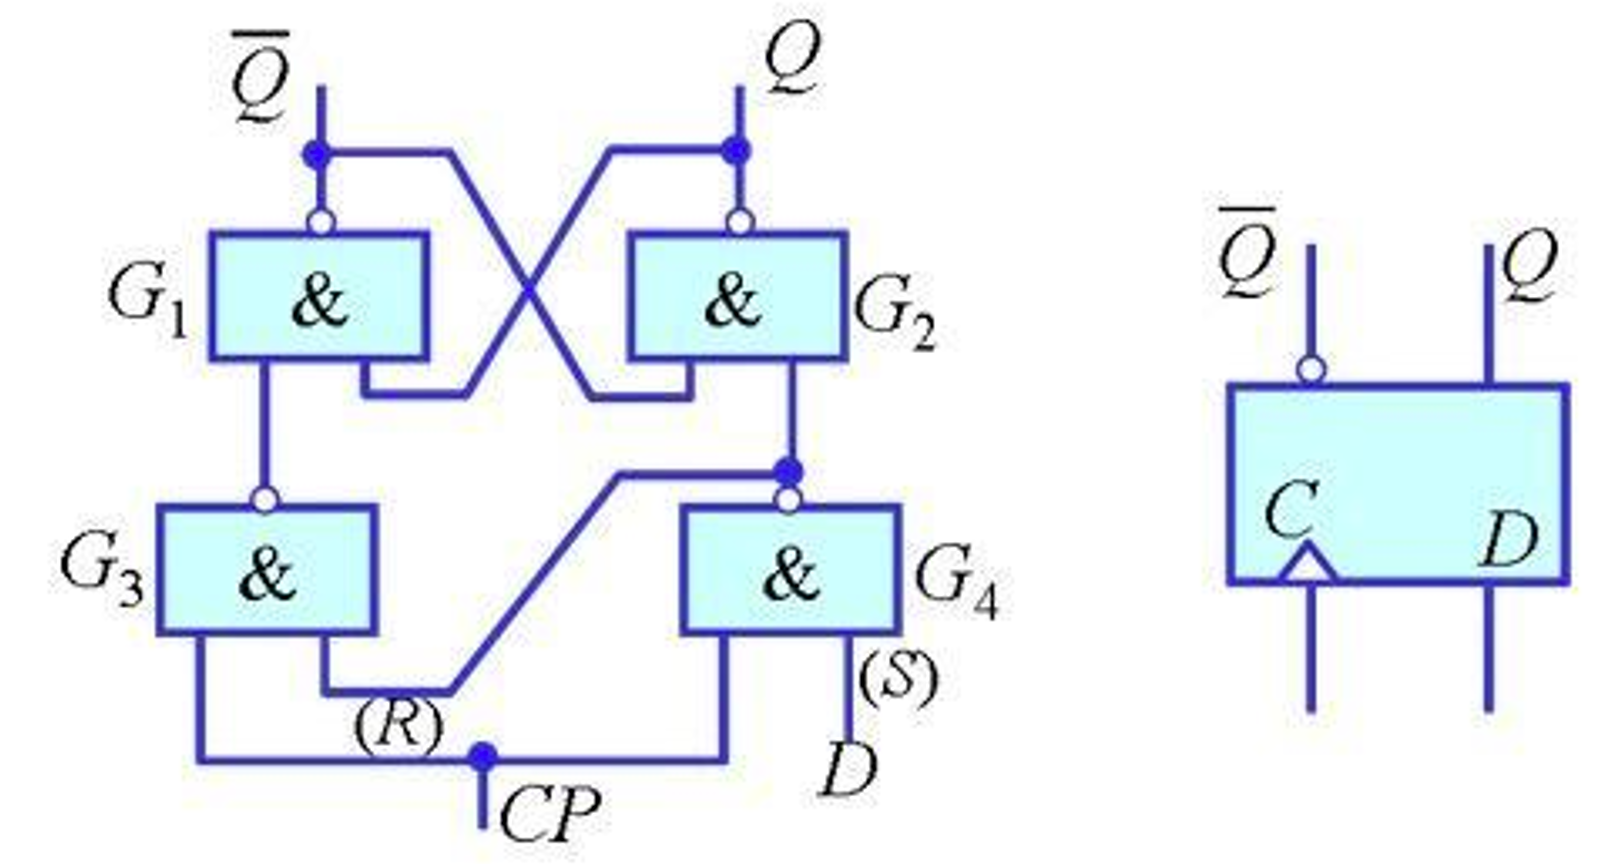
\includegraphics[height=3.5cm]{fig/D_flip_flop.png}
                    \caption{D触发器结构图}
                    \label{fig:D_flip_flop}
                \end{minipage}
                \quad
                \begin{minipage}{0.4\linewidth}
                    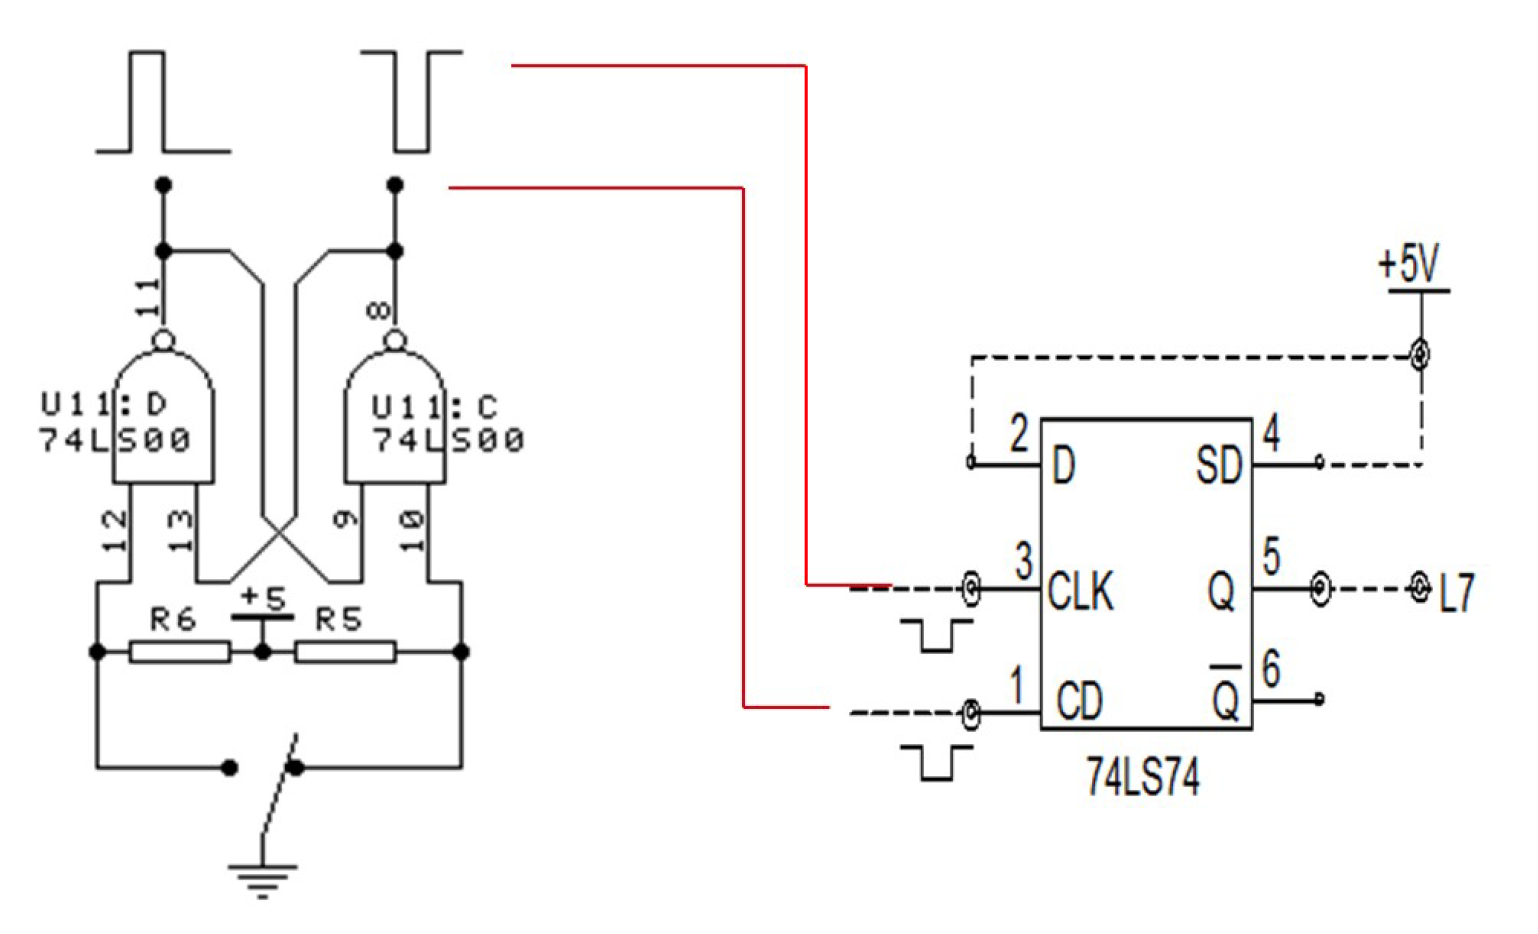
\includegraphics[height=3.5cm]{fig/D_test.png}
                    \caption{D触发器基本特性测量电路}
                    \label{fig:D_test}
                \end{minipage}
            \end{figure}

        \subsection{环形振荡器}

            环形振荡器的原理图如图~\ref{subfig:oscillation_init}~所示,由于实验箱与门、或门、非门各仅有一个,所以需要使用图~\ref{subfig:oscillation_real}~所示电路来等效.
            此处震荡是靠门延时来实现,每经过一个门输出 $F=\overline{y}$.

            \begin{figure}[htbp]
                \centering
                \subfloat[原理图]{
                    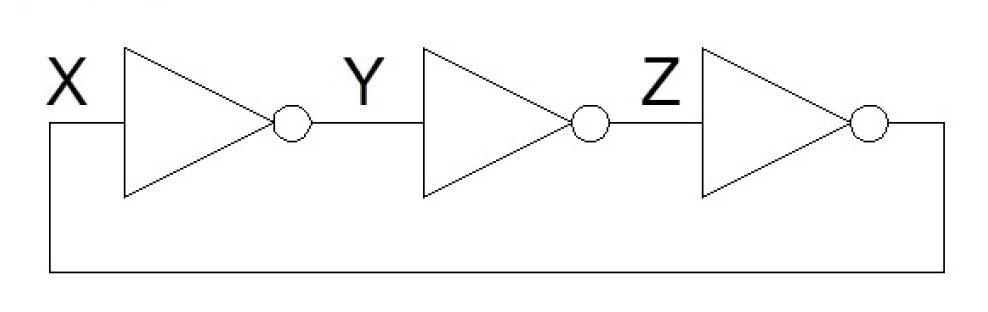
\includegraphics[height=2cm]{fig/oscillation_init.png}
                    \label{subfig:oscillation_init}
                }
                \subfloat[等效图]{
                    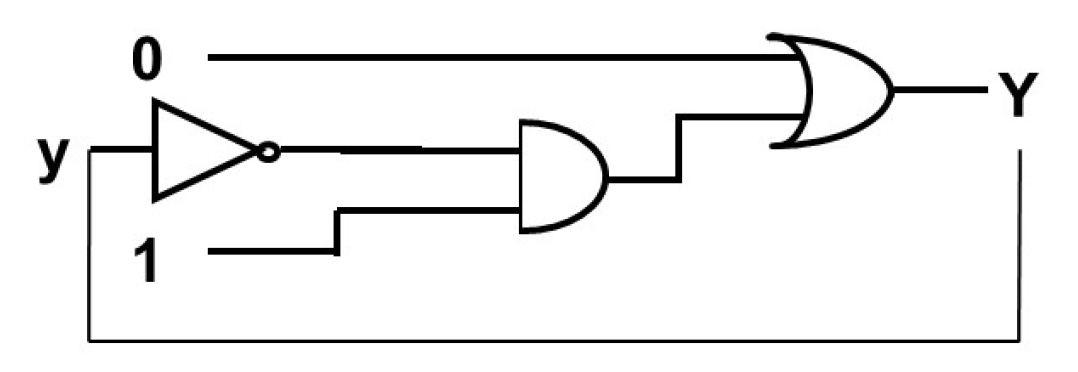
\includegraphics[height=2cm]{fig/oscillation_real.png}
                    \label{subfig:oscillation_real}
                }
                \caption{环形振荡器电路图}
                \label{fig:oscillation_circuit}
            \end{figure}

            \vspace{-1cm}

    \section{方案实现与测试}

        \subsection{信号源和示波器}

            RIGOL DG1022U25MHz 双路波形发生器和 RIGOL DS1072E-EDU
            70MHz 双踪数字记忆示波器的操作使用.

            图~\ref{subfig:square_32.47k}, \ref{subfig:square_1k}, \ref{subfig:square_1}~分别是$32.768\mathrm{kHz}$、$1\mathrm{kHz}$ 和 $1\mathrm{Hz}$ 时示波器观察到的波形.

            \begin{figure}[htbp]
                \centering
                \subfloat[$32.768\mathrm{kHz}$]{
                    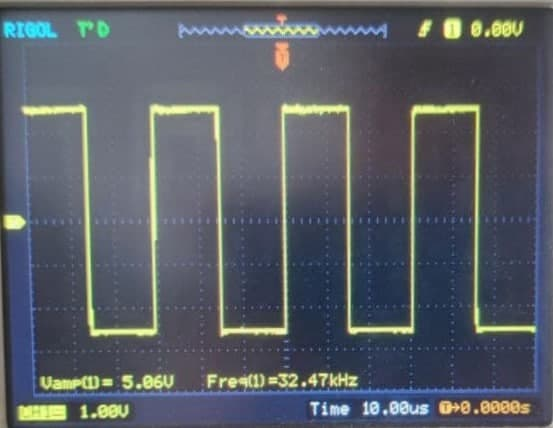
\includegraphics[height=4cm]{fig/square_32.47k.jpg}
                    \label{subfig:square_32.47k}
                }
                \subfloat[$1\mathrm{kHz}$]{
                    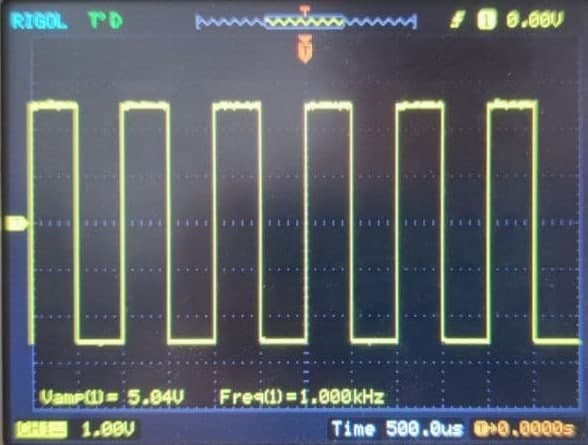
\includegraphics[height=4cm]{fig/square_1k.jpg}
                    \label{subfig:square_1k}
                }
                \subfloat[$1\mathrm{Hz}$]{
                    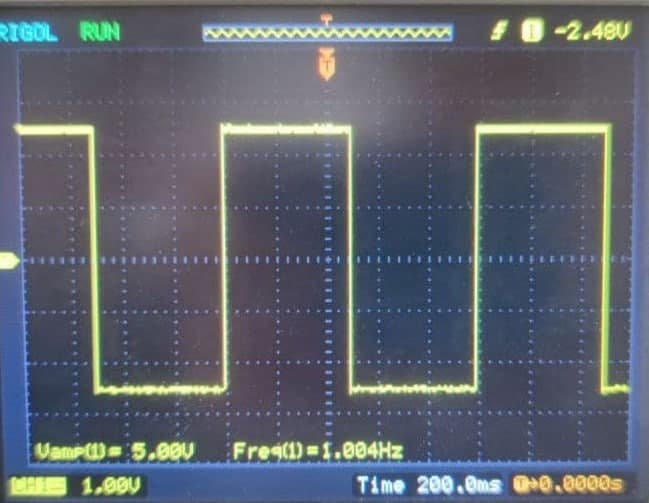
\includegraphics[height=4cm]{fig/square_1.jpg}
                    \label{subfig:square_1}
                }
                \caption{高低电平方波的示波器显示}
                \label{fig:square_wave}
            \end{figure}

            \begin{note}{示波器的使用}{use_oscilloscope}
                示波器使用时需要和输入信号\textbf{共地},
                否则可能会有很大的区别(例如,不接入任何有效电压的时候可以观测到 $50\mathrm{Hz}$的信号波动),虽然由于仪器可能共用拖线板达到了共抵的效果.
            \end{note}

        \subsection{D触发器控制LED}

            通过与门、或门、非门,控制LED灯的亮和灭,具体电路如图~\ref{fig:LED}~所示.
            实验结果与理论的亮灭情况一致.

            \begin{figure}[htbp]
                \centering
                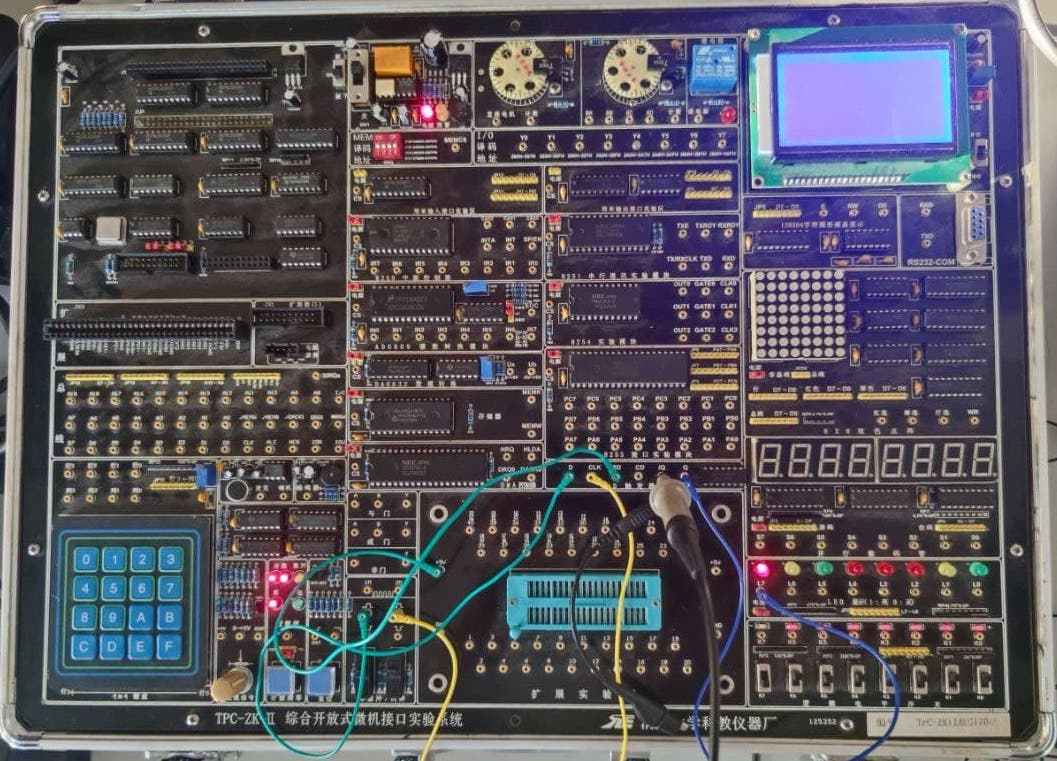
\includegraphics[width=.6\linewidth]{fig/LED.jpg}
                \caption{D触发器控制LED的实际电路}
                \label{fig:LED}
            \end{figure}

        \subsection{8段数码管的显示}

            通过电路连接可以做到8段数码管的显示,如图~\ref{fig:digit_LED}~所示.
            我们通过排线让所有的位有同样的数字显示.

            \begin{figure}[htbp]
                \centering
                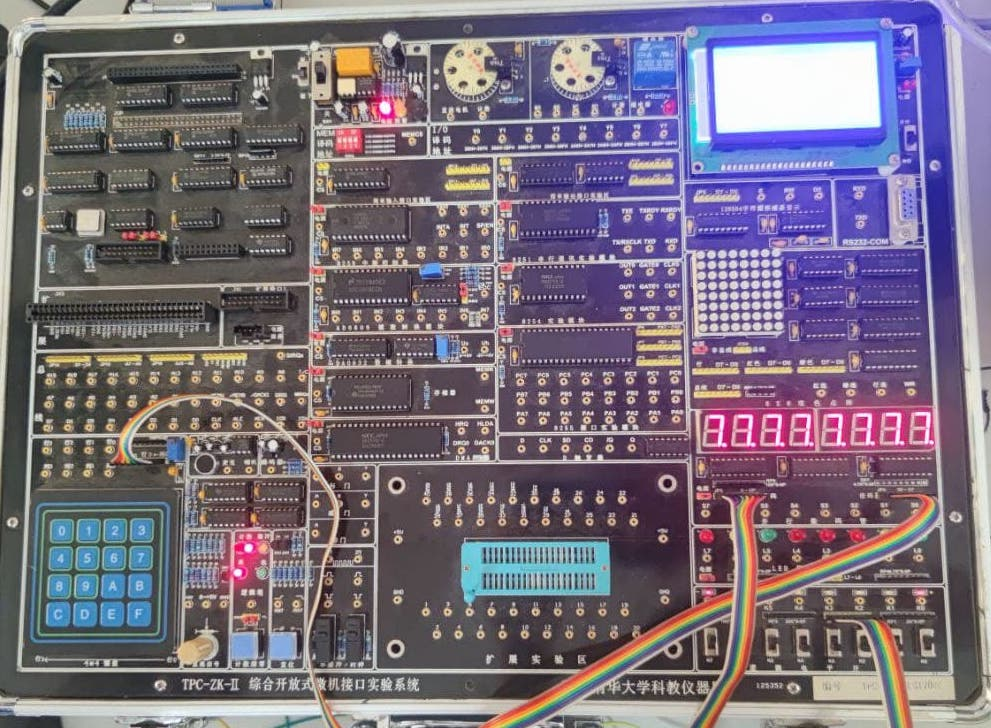
\includegraphics[width=.6\linewidth]{fig/Digit_LED.jpg}
                \caption{8段数码管显示的实际电路}
                \label{fig:digit_LED}
            \end{figure}

        \subsection{环形振荡器}

            环形振荡器电路按照图~\ref{subfig:oscillation_real}~搭建,
            通过示波器可以看到震荡的效果(如图~\ref{fig:two_waves}~所示),两个通道之间的相位差可以清晰的看到.

            \begin{figure}[htbp]
                \centering
                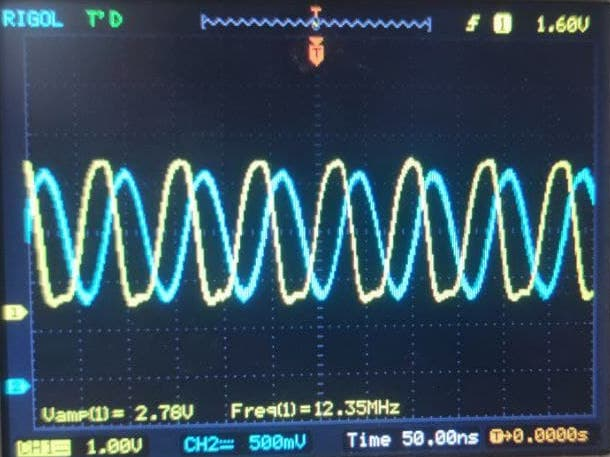
\includegraphics[width=.4\linewidth]{fig/two_waves.jpg}
                \caption{环形振荡器示波器波形显示}
                \label{fig:two_waves}
            \end{figure}

            \begin{note}{环形振荡器}{}
                实验前需要\textbf{检验设备},这很重要!
                我们的实验过程中电路经过检查没有问题,最终发现与门存在故障,
                不管输入电平如何输出永远都是高电平.
            \end{note}

        \subsection{Vivado 开发初探}

            \begin{device}{Vivado 实验器材}{vivado}
                \begin{itemize}
                    \item Xilinx Vivado \textit{HLx} 2017.4
                    \item Ubuntu 20 / Windows 11 (x86\_64){\kaishu\color{gray}(主要实验于 Ubuntu 平台完成)}
                    \item 没有具体的开发板,仅限于线上仿真和使用 Verilog 进行电路设计
                \end{itemize}
            \end{device}

            \subsubsection{行为仿真}

                通过行为仿真(\texttt{behavioral simulation}),我们可以观测到图~\ref{fig:behavioral_simulation}~中的结果.
                \texttt{switches[7:0]}的结果基本可以说明其计数器的功能.
                调整如下代码中第5行的延时,即修改计数一次维持的时间,而第6行的延时则是改变上升沿的时间.

                \begin{lstlisting}[language=verilog,title=tutorial\_tb.v]
initial
begin
    for (i = 0; i < 255; i = i+2)
    begin
        #50 switches=i; // time for each step
        #10 e_led = expected_led(switches); // transition time
        if (leds == e_led)
            $display ("LED output matched at", $time);
        else
            $display ("LED output mis-matched at ", $time,": expected: %b, actual: %b", e_led, leds);
    end
end
                \end{lstlisting}

                \begin{analyze}{时延的影响}{}
                    上述代码中的实验控制可以理解为梯形的几个几何参数:上底长度和其腰的投影长度.
                \end{analyze}

                \begin{note}{行为仿真的查看}{}
                    注意图~\ref{fig:behavioral_simulation}~中观测行为仿真需点开数组(例如\texttt{switches}和\texttt{leds}),
                    另外需要将窗口展示的范围调整到合适的值.
                \end{note}

                \begin{figure}[htbp]
                    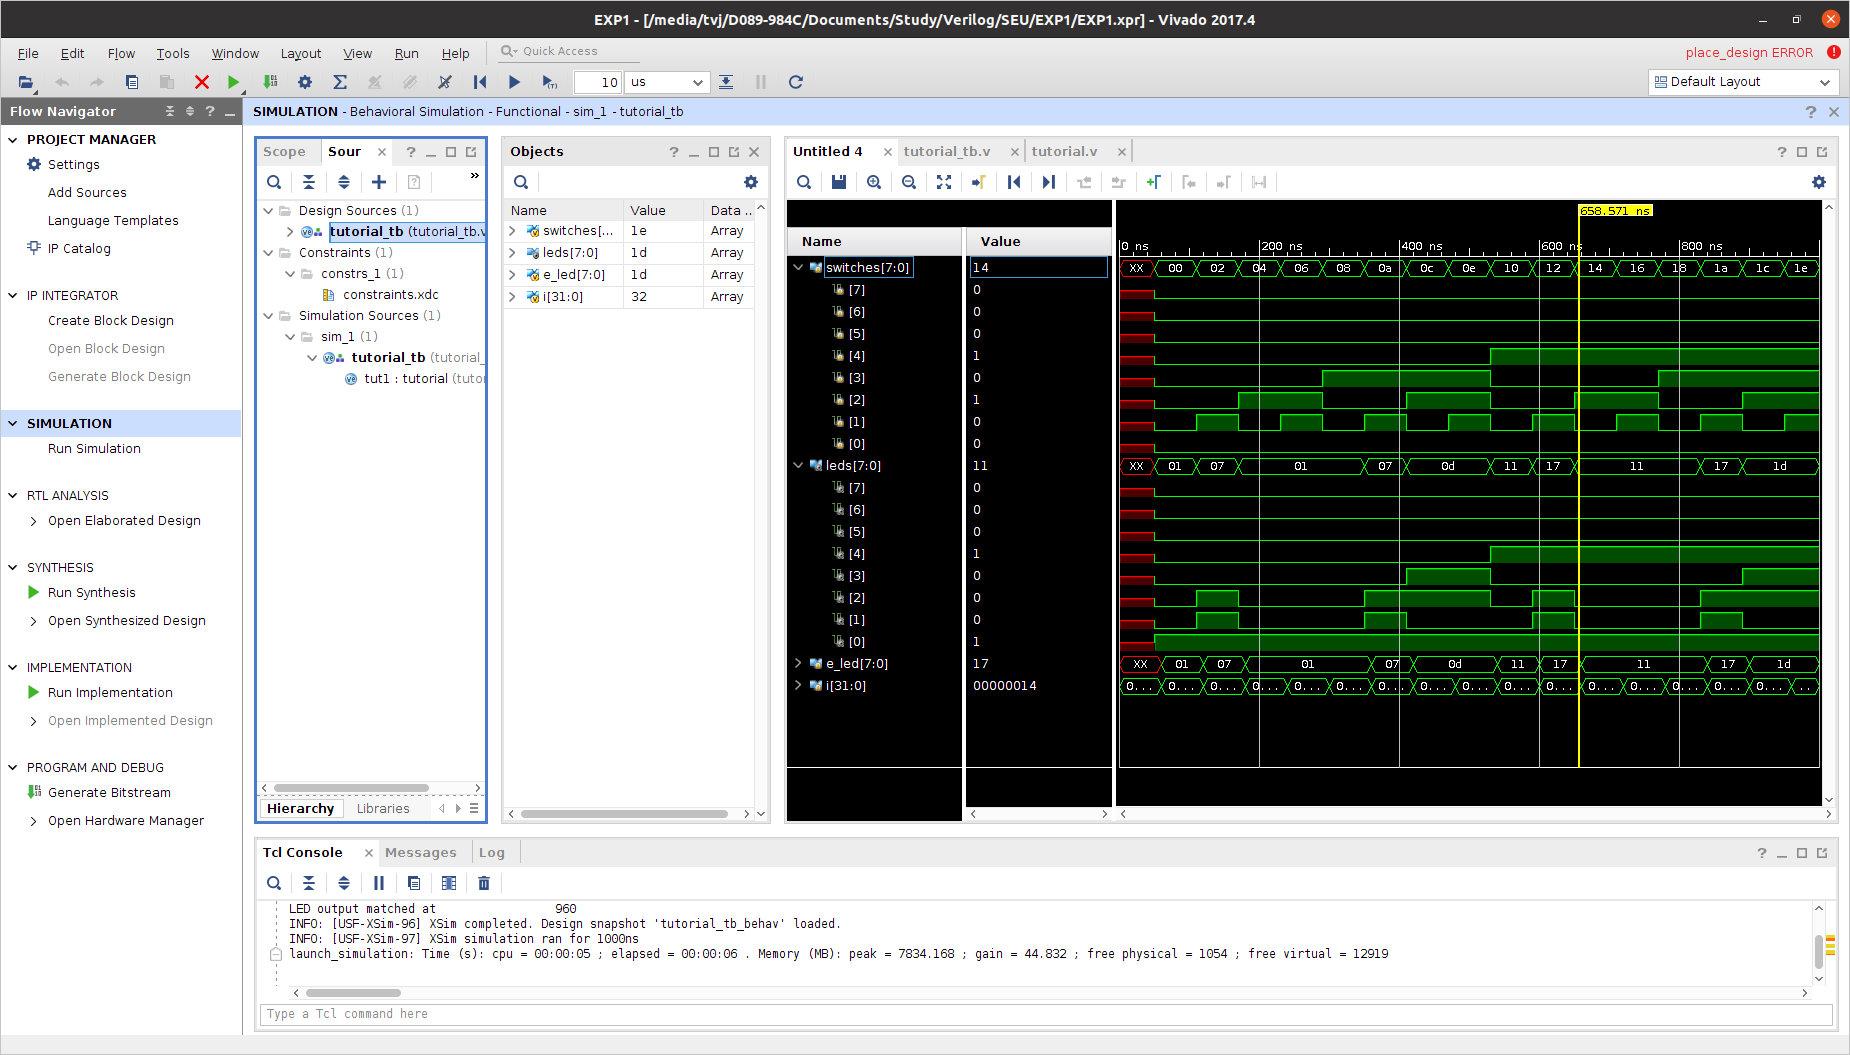
\includegraphics[width=\linewidth]{fig/behavioral_simulation_EXP1.png}
                    \caption{行为仿真图(tutorial)}
                    \label{fig:behavioral_simulation}
                \end{figure}

            \subsubsection{RTL级电路}

                通过 \texttt{run synthesis} 可以获得电路的 RTL 级电路.
                图~\ref{subfig:RTL_tff}~保留了完整的\texttt{tff}\footnote{代码来自\cite{github:fpga-verilog}.}模块,不过也可以像图~\ref{subfig:RTL_EXP1}~一样展开模块的内容.

                \begin{figure}[htbp]
                    \centering
                    \subfloat[tff]{
                        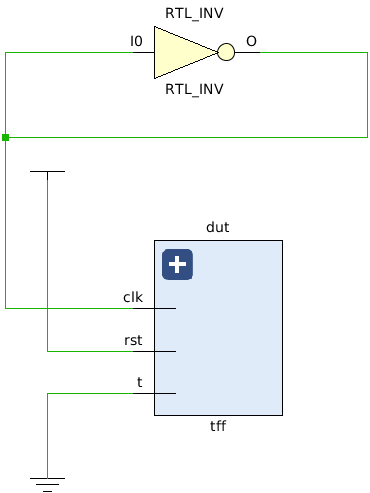
\includegraphics[height=6.5cm]{fig/RTL_tff.png}
                        \label{subfig:RTL_tff}
                    }\hfill
                    \subfloat[tutorial]{
                        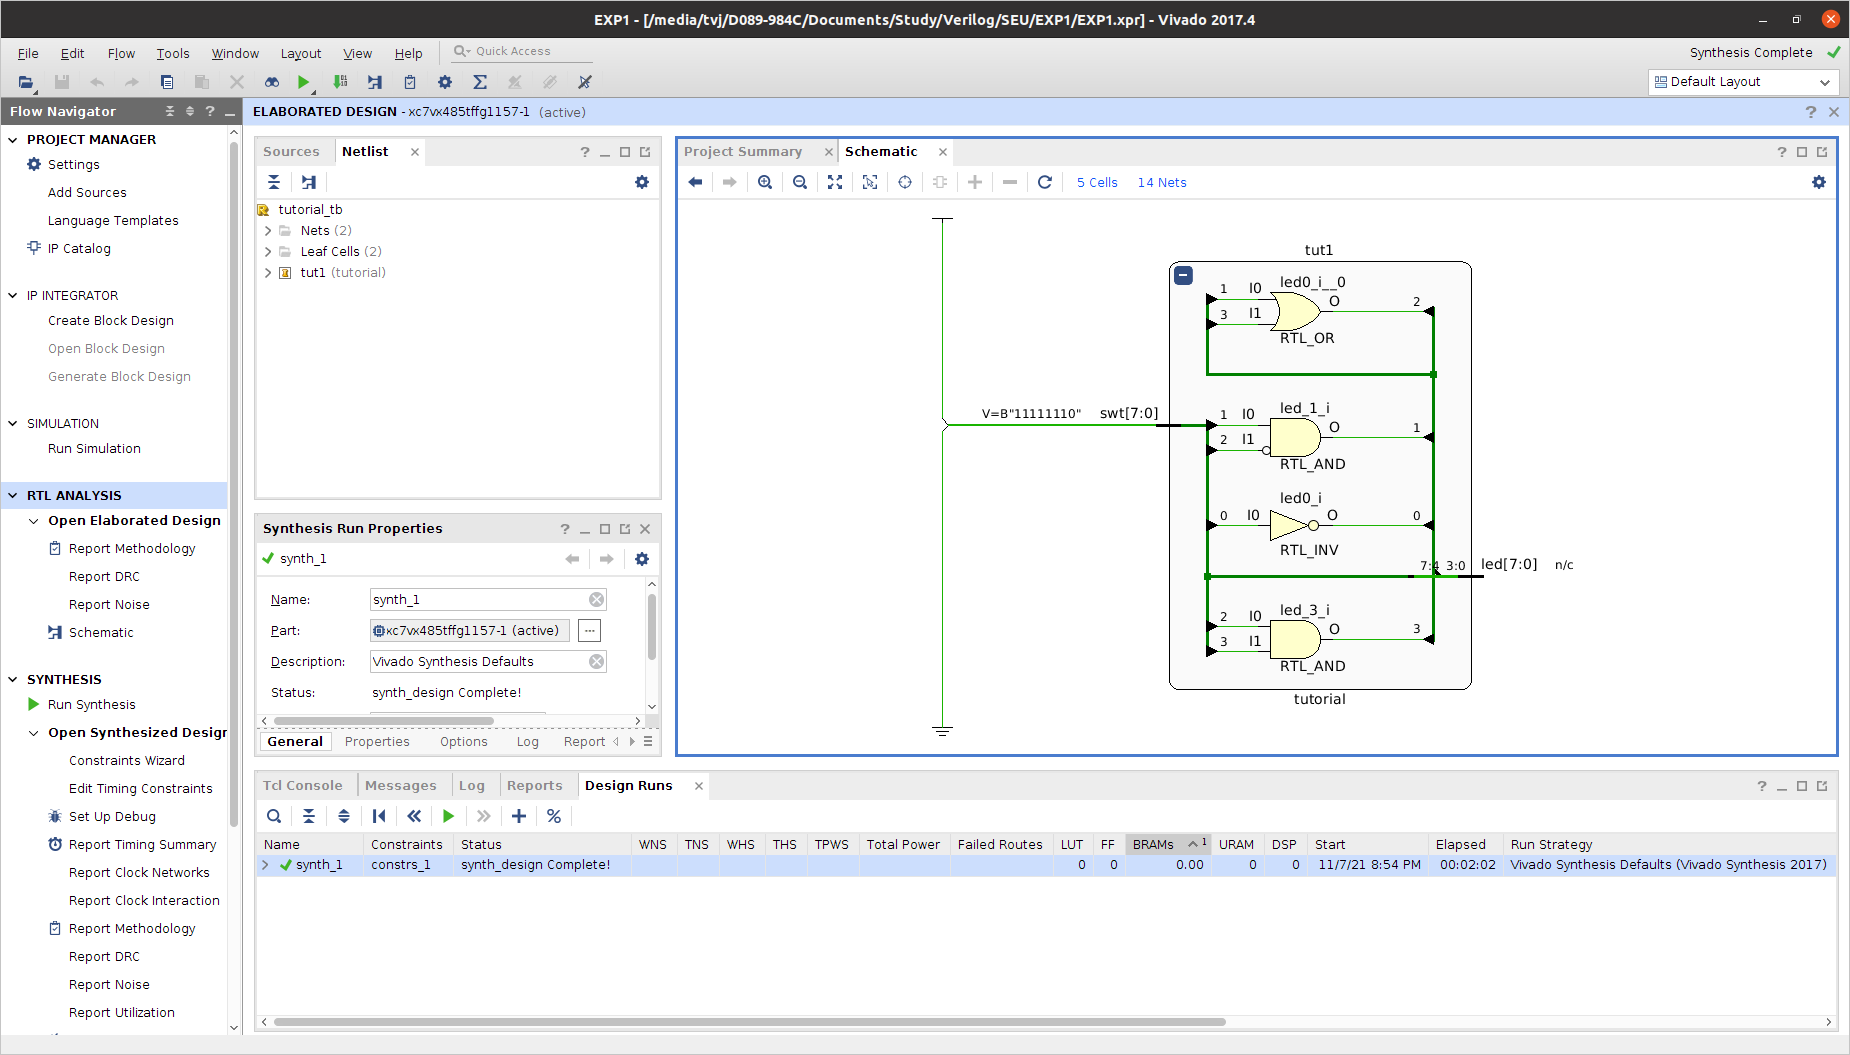
\includegraphics[height=6.5cm]{fig/RTL_EXP1.png}
                        \label{subfig:RTL_EXP1}
                    }
                    \caption{RTL级电路}
                    \label{fig:RTL}
                \end{figure}

            \subsubsection{硬件实现}

                通过添加约束文件(\texttt{constraint}),
                对硬件的结构(例如引脚)做出约束,
                然后 \texttt{run implementation},
                得到例如图~\ref{fig:implementation}~的复杂电路.
                不过由于没有具体的开发板,后面的步骤无法继续进行,
                目前只做了了解.

                \begin{figure}[h!]
                    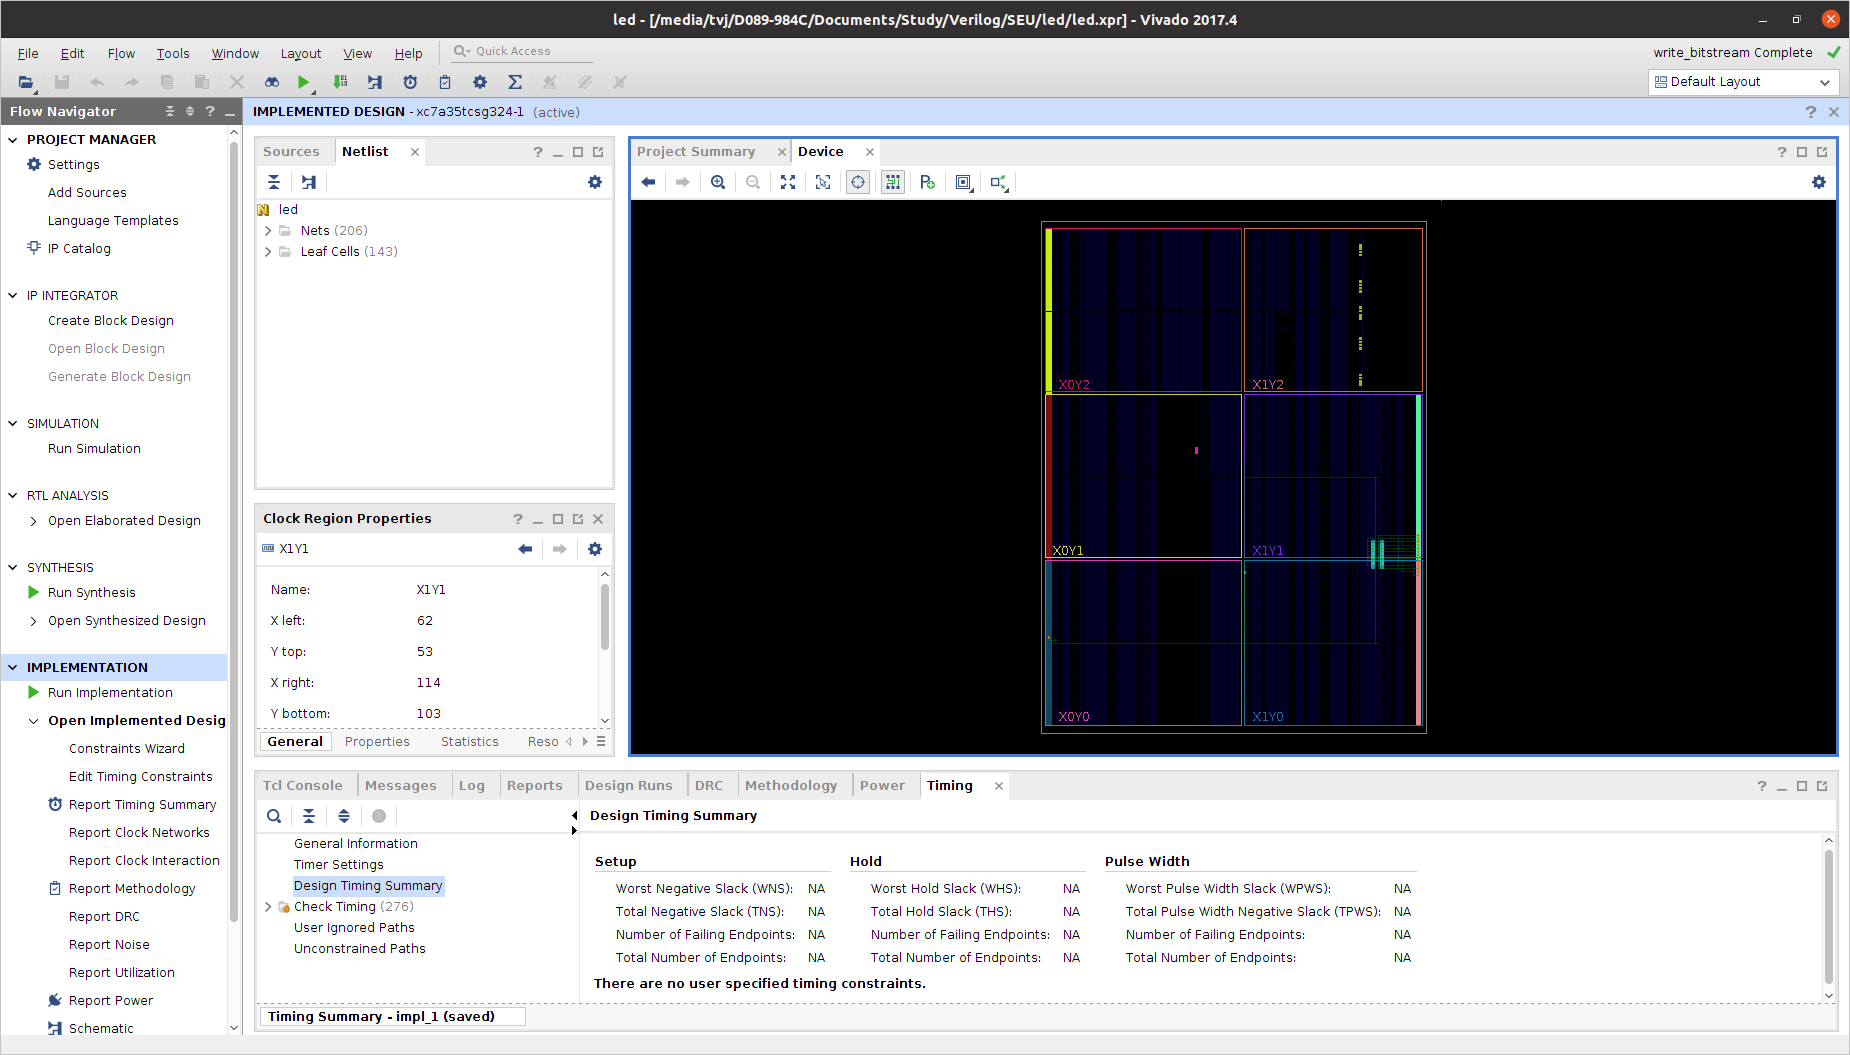
\includegraphics[width=\linewidth]{fig/implementation.png}
                    \caption{硬件实现(led)}
                    \label{fig:implementation}
                \end{figure}

            \subsubsection{其他工作}

                \texttt{led.v} 的 RTL 级电路图为图~\ref{fig:RTL_led}.

                \begin{figure}[htbp]
                    \centering
                    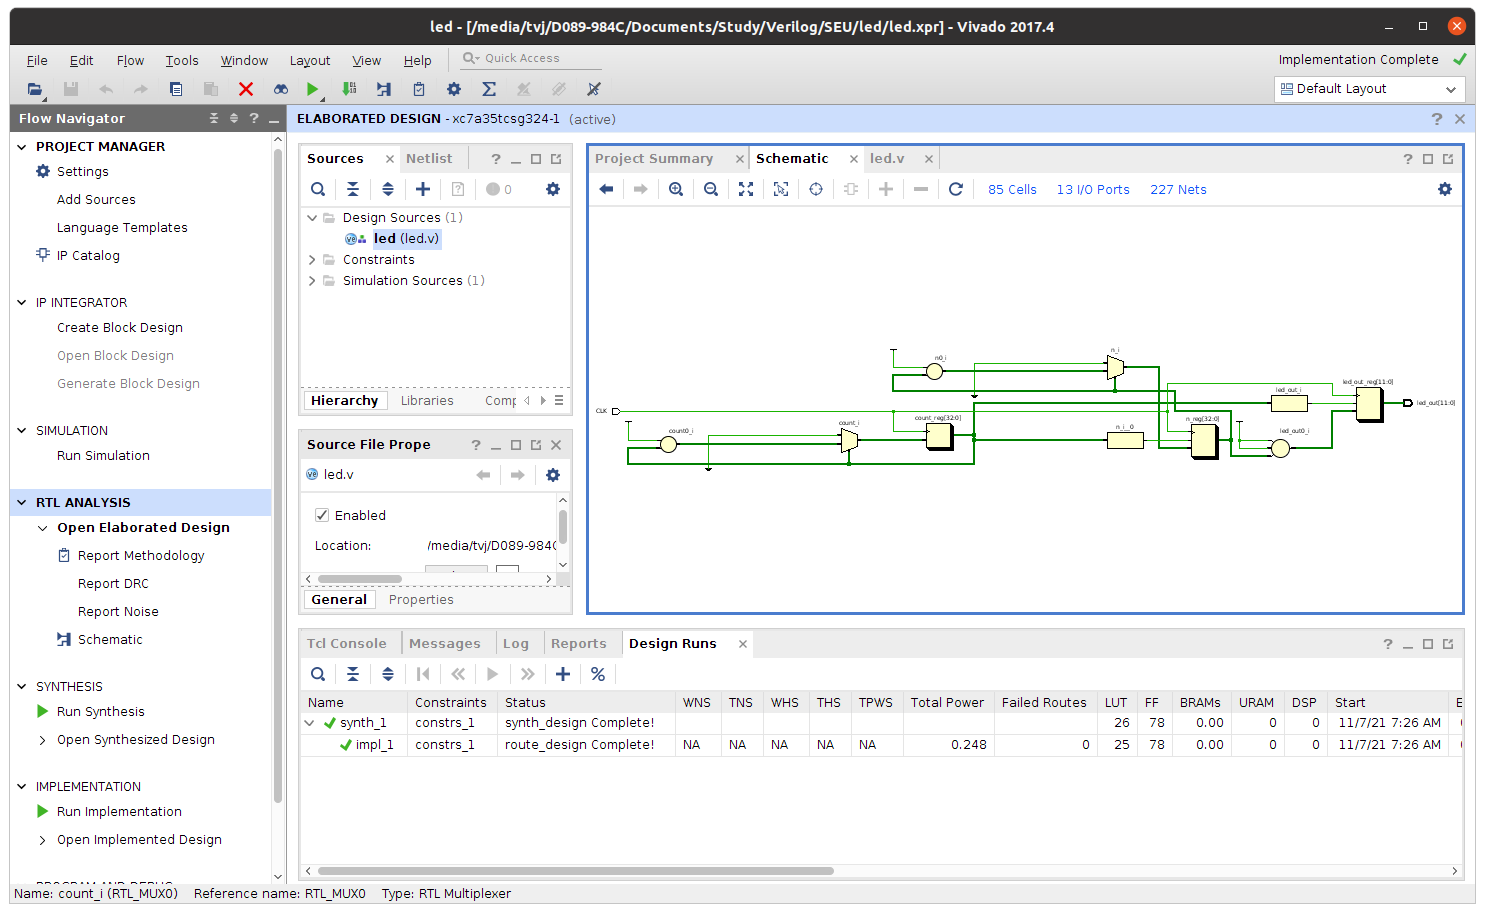
\includegraphics[width=.75\linewidth]{fig/RTL_led.png}
                    \caption{RTL 级电路(led)}
                    \label{fig:RTL_led}
                \end{figure}

                另外一部分工作详见第~\ref{sec:improvenment}~章第~\ref{subsec:vivado_improvement}~节.

    \section{提高与创新研究}\label{sec:improvenment}

        \subsection{双色点阵发光二极管显示控制}

            通过连接电路,我们控制了双色点阵发光二极管的显示,效果如图~\ref{fig:LEDs}~所示,每一次变化除了需要调节开关,还需要控制单脉冲电路以激活状态.

            \begin{figure}[htbp]
                \centering
                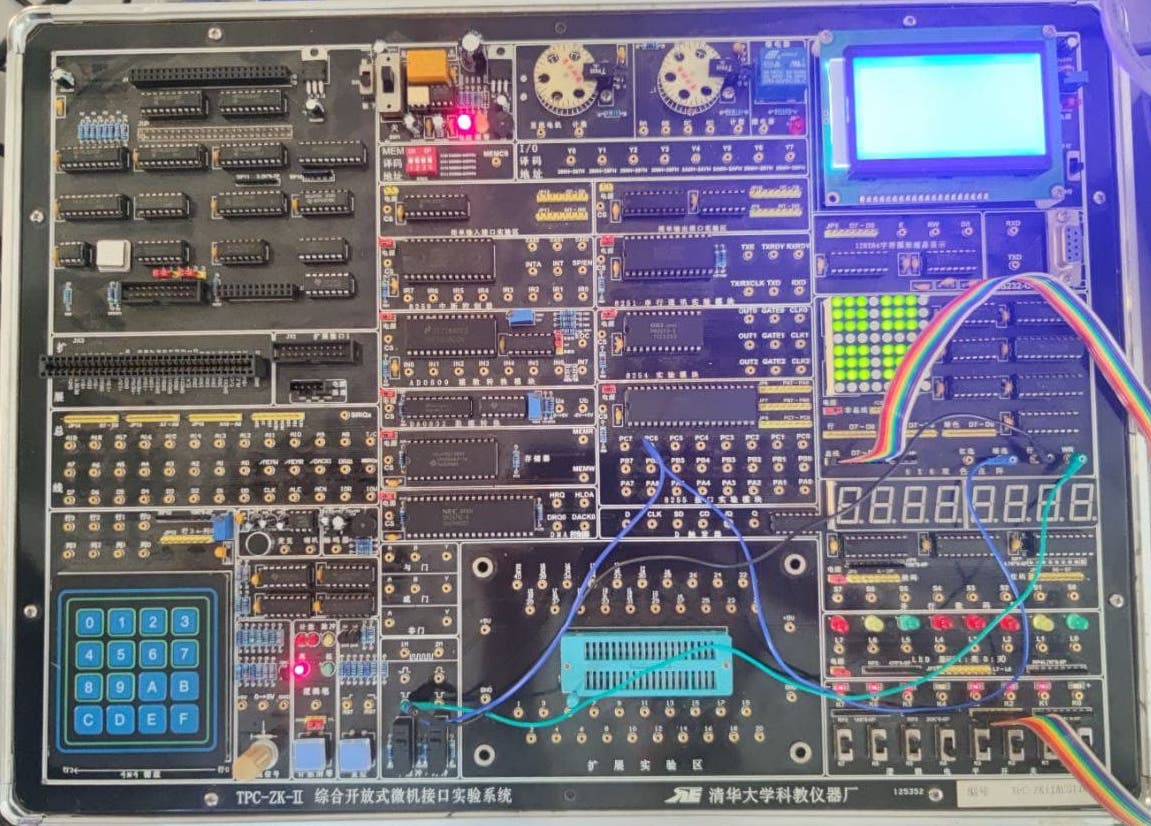
\includegraphics[width=.6\linewidth]{fig/LEDs.jpg}
                \caption{双色点阵发光二极管的显示控制电路}
                \label{fig:LEDs}
            \end{figure}

        \subsection{Vivado 开发设计}\label{subsec:vivado_improvement}

            我主要通过\texttt{tff}\cite{github:fpga-verilog}的代码对 Vivado 做了更深的了解.

            \begin{idea}{Vivado 层次调用}{vivado_levels}
                此处有\texttt{tff\_tb.v} (test bench) 和核心模块\texttt{tff.v},test bench 通过创建一个 \texttt{tff} 类变量即可实现调用,体现在 schematic 图(图~\ref{fig:RTL})上即一个可以展开或收起对框.

                下面是 test bench 的代码.
                \begin{lstlisting}[numbers=none,language=verilog,title=tff\_tb.v,backgroundcolor=\color{blue!3},morekeywords={tff}]
module tff_tb;
    reg clk, reset, t;
    wire q;
    tff dut (.clk(clk), .t(t), .rst (reset), .q(q));
    
    initial clk = 1'b0;
    always #5 clk = ~clk; // clock generation
    
    initial
    begin
        reset = 1'b1;
        t = 1'b1;
        #20 reset = 1'b0; 
        #50 t = 1'b0;
        #30 reset = 1'b1;
        #30 $stop;
    end
endmodule
                \end{lstlisting}
                下面是\texttt{tff}的核心代码.
                \begin{lstlisting}[numbers=none,language=verilog,title=tff.v,backgroundcolor=\color{blue!3}]
module tff(
    input clk, rst, t,
    output reg q, 
    output qb
    );
    always @ (posedge clk, posedge rst)  // asynchronous reset
    begin
        if (rst)
            q <= 1'b0;
        else if (t)
            q <= ~q;
        else 
            q <= q;
    end  
    assign qb = ~q;
endmodule
            \end{lstlisting}
            \end{idea}

            \begin{idea}{Vivado 整体设计思路}{}
                从思考~\ref{idea:vivado_levels}~中总结,可以得到 Vivado 设计的总体思路.
                Vivado 在结构上类似 C++,
                能够定义\textbf{类}来实现\textbf{层次的堆叠}.
                因此 Vivado 项目是基于众多 components 的,
                而这些 components 既可以来源于 Verilog 标准(相当于 C 语言),
                又可以来自例如\texttt{xup}库(相当于 C++ 标准库)等地方,当然我们也可以自己定义我们的类.

                我的导师在研究生阶段研究极化码(polar codes),其中极化码 BP 译码(belief propagation)架构从 butterfly 结构层层向上加,结构清晰且易于证明架构的正确性.
            \end{idea}

    \section{分析与总结}

        具体的问题与思考在对应的位置已有分析,
        此处主要阐述对实验总体的体悟.

        我目前对于算法的研究较多(例如在课题组的工作方向是``智能反射表面的信道估计"),而在硬件实现的能力上有所欠缺.
        一方面,需要较强的动手操作能力,另一方面,硬件设计是一个和算法相差很多的工作领域,虽然关联非常密切,但需要考虑的问题会和算法有一定的出入.

        不过目前我还能较好适应这样的工作内容,经过锻炼,一方面是学习到了``如何独立自主学习"的技能,另一方面在利用代码能力优势的同时加强代码与硬件联系的能力,最后在成果总结(例如文字总结和 \LaTeX 技巧)上也有不小的提升.

        在下一阶段,我将对 Vivado (Verilog) 做更深入的了解.

    % 打印参考文献
    \addcontentsline{toc}{section}{参考文献}
    \printbibliography

    \newpage
    \addcontentsline{toc}{section}{附录:实验报告 \LaTeX 模板}
    \section*{附录:实验报告 \LaTeX 模板}

        实验报告使用自己编写的 \LaTeX 模板(\texttt{SEU-Digital-Report.cls}),
        在基本适配 Microsoft Word 版报告的格式要求之外,
        增加了更多的功能,使得报告看起来更加优雅多彩.

        后续升级后,报告模板将于 \url{https://github.com/Teddy-van-Jerry/TVJ-Digital-Report} 基于 MIT License 开源共享.

        编译需要使用 \texttt{XeLaTeX + Biber},封面页修改如下内容即可.
        \begin{lstlisting}[
            language=tex,
            morekeywords={
                expno,
                expname,
                expauthor,
                expID,
                expmates,
                expmatesID,
                expmajor,
                explab,
                expdate,
                expreportdate,
                expgrade,
                exptutor,
                today
            }
        ]
%%%%%%%%%%%%%%%%%%%% 报告基本信息 %%%%%%%%%%%%%%%%%%%%
\expno{一} % 实验序号
\expname{数字逻辑与实验环境认识} % 实验名称
\expauthor{赵舞穹} % 姓名
\expID{61520522} % 学号
\expmates{郑瑞琪} % 同组
\expmatesID{61520523} % 学号(同组)
\expmajor{工科试验班} % 专业
\explab{计算机硬件技术} % 实验室
\expdate{2021年10月29日} % 实验日期
\expreportdate{\today} % 实验日期
\expgrade{} % 成绩评定
\exptutor{冯熳} % 评阅教师
%%%%%%%%%%%%%%%%%%%%%%%%%%%%%%%%%%%%%%%%%%%%%%%%%%%%
        \end{lstlisting}

\end{document}
